% This file was created by tikzplotlib v0.9.8.
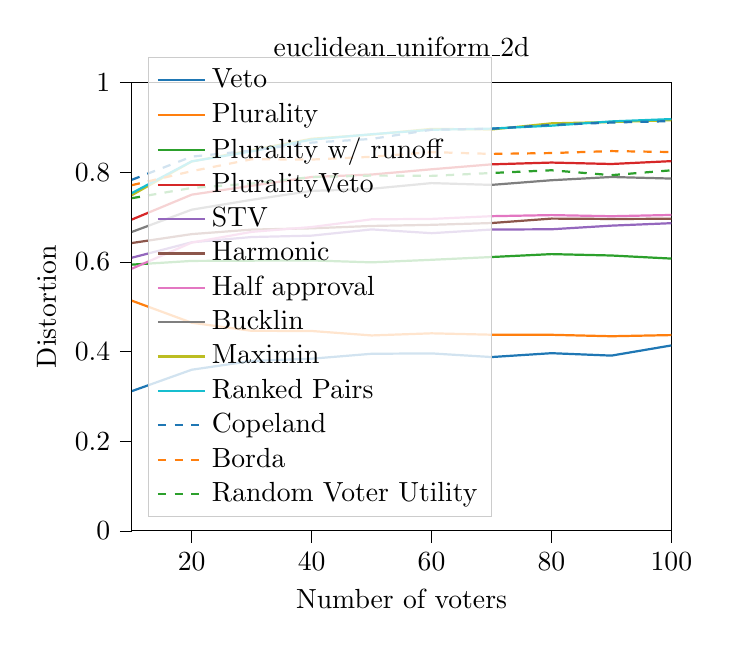
\begin{tikzpicture}

\definecolor{color0}{rgb}{0.12156862745098,0.466666666666667,0.705882352941177}
\definecolor{color1}{rgb}{1,0.498039215686275,0.0549019607843137}
\definecolor{color2}{rgb}{0.172549019607843,0.627450980392157,0.172549019607843}
\definecolor{color3}{rgb}{0.83921568627451,0.152941176470588,0.156862745098039}
\definecolor{color4}{rgb}{0.580392156862745,0.403921568627451,0.741176470588235}
\definecolor{color5}{rgb}{0.549019607843137,0.337254901960784,0.294117647058824}
\definecolor{color6}{rgb}{0.890196078431372,0.466666666666667,0.76078431372549}
\definecolor{color7}{rgb}{0.737254901960784,0.741176470588235,0.133333333333333}
\definecolor{color8}{rgb}{0.0901960784313725,0.745098039215686,0.811764705882353}

\begin{axis}[
legend cell align={left},
legend style={
  fill opacity=0.8,
  draw opacity=1,
  text opacity=1,
  at={(0.03,0.03)},
  anchor=south west,
  draw=white!80!black
},
tick align=outside,
tick pos=left,
title={euclidean\_uniform\_2d},
x grid style={white!69.0196078431373!black},
xlabel={Number of voters},
xmin=10, xmax=100,
xtick style={color=black},
y grid style={white!69.0196078431373!black},
ylabel={Distortion},
ymin=0, ymax=1,
ytick style={color=black}
]
\addplot [thick, color0]
table {%
10 0.3115
20 0.3593
30 0.3789
40 0.3839
50 0.3949
60 0.3957
70 0.3876
80 0.3962
90 0.3908
100 0.4135
};
\addlegendentry{Veto}
\addplot [thick, color1]
table {%
10 0.5134
20 0.4641
30 0.4461
40 0.4457
50 0.4358
60 0.4405
70 0.4374
80 0.4372
90 0.434
100 0.4366
};
\addlegendentry{Plurality}
\addplot [thick, color2]
table {%
10 0.5937
20 0.602
30 0.6026
40 0.6031
50 0.5988
60 0.6045
70 0.6107
80 0.6172
90 0.6141
100 0.6072
};
\addlegendentry{Plurality w/ runoff}
\addplot [thick, color3]
table {%
10 0.6942
20 0.7498
30 0.7697
40 0.7892
50 0.7947
60 0.8064
70 0.8174
80 0.8214
90 0.8182
100 0.8246
};
\addlegendentry{PluralityVeto}
\addplot [thick, color4]
table {%
10 0.6091
20 0.6436
30 0.6553
40 0.6584
50 0.6723
60 0.6639
70 0.672
80 0.6726
90 0.6807
100 0.6862
};
\addlegendentry{STV}
\addplot [thick, color5]
table {%
10 0.6419
20 0.6618
30 0.6719
40 0.6747
50 0.68
60 0.6825
70 0.6865
80 0.6964
90 0.6956
100 0.696
};
\addlegendentry{Harmonic}
\addplot [thick, color6]
table {%
10 0.5846
20 0.6429
30 0.6668
40 0.6776
50 0.6948
60 0.6957
70 0.7018
80 0.7042
90 0.7017
100 0.7045
};
\addlegendentry{Half approval}
\addplot [thick, white!49.8039215686275!black]
table {%
10 0.6666
20 0.7163
30 0.7383
40 0.7581
50 0.7629
60 0.7756
70 0.7716
80 0.782
90 0.7892
100 0.7857
};
\addlegendentry{Bucklin}
\addplot [thick, color7]
table {%
10 0.7486
20 0.8238
30 0.8491
40 0.8745
50 0.8838
60 0.8965
70 0.8952
80 0.9089
90 0.9118
100 0.9159
};
\addlegendentry{Maximin}
\addplot [thick, color8]
table {%
10 0.7532
20 0.8241
30 0.8463
40 0.8727
50 0.8846
60 0.8945
70 0.8972
80 0.9037
90 0.9132
100 0.9184
};
\addlegendentry{Ranked Pairs}
\addplot [thick, color0, dashed]
table {%
10 0.7829
20 0.8346
30 0.8483
40 0.8659
50 0.8741
60 0.8947
70 0.8969
80 0.9052
90 0.9107
100 0.9139
};
\addlegendentry{Copeland}
\addplot [thick, color1, dashed]
table {%
10 0.7709
20 0.8022
30 0.8288
40 0.8281
50 0.8343
60 0.8447
70 0.8407
80 0.8426
90 0.847
100 0.8449
};
\addlegendentry{Borda}
\addplot [thick, color2, dashed]
table {%
10 0.7419
20 0.7648
30 0.7746
40 0.7891
50 0.7924
60 0.7917
70 0.7981
80 0.8042
90 0.7933
100 0.8041
};
\addlegendentry{Random Voter Utility}
\end{axis}

\end{tikzpicture}
